% !TeX spellcheck = it_IT
%!TEX encoding = UTF-8 Unicode
%Author: Fulvio Frapolli
%Last revision: 06.09.2019
\documentclass[
%todo,
%answers,
finale,
%sectnum,
ssectnum,
%twocolumn,
]{DossierExMathIta}

\titolo[indice]{Database}
%\titolo{PAP1}
\author{CPT}
\date{2020}


%\pgfplotsset{AxisDefaults/.append style={width=\linewidth,}}
\tikzstyle{every node}=[font=\footnotesize] 
%\partlabel{\arabic{partno})} %% Keep consistency in part numbering  with the screenshots

\makeatletter
\def\input@path{{esercizi/}{temi/}}
%or: \def\input@path{{/path/to/folder/}{/path/to/other/folder/}}
\makeatother



\includeonly{temi/31.grado1}


\begin{document}
\setlength{\columnsep}{0.6cm}
\indice


\section{Insiemi}
\subsection{Numeri}
\begin{questions}

\question

\exonly{	Indica a quali insiemi appartengono i seguenti valori: }

\begin{minipage}{\linewidth}
	\begin{multicols}{2}
		\begin{tabular}{|c|c|c|c|c|}
			\hline
			& $ \mathbb{N}$ & $ \mathbb{Z}  $ & $ \mathbb{Q}$ & $ \mathbb{R} $ \\
			\hline
			$ 4 $      &      \solonly{\checkmark }         &  \solonly{\checkmark }                &    \solonly{\checkmark }            &    \solonly{\checkmark }             \\
			\hline
			$ -0.34 $    &               &                 &    \solonly{\checkmark }            &      \solonly{\checkmark }           \\
			\hline
			$ -71 $     &               &      \solonly{\checkmark }            &    \solonly{\checkmark }            &   \solonly{\checkmark }              \\
			\hline
			$ \frac{3}{4} $ &               &                 &     \solonly{\checkmark }           &        \solonly{\checkmark }         \\
			\hline
			$ \pi $     &               &                 &               &    \solonly{\checkmark }             \\
			\hline
			$ \sqrt{2} $   &               &                 &               &    \solonly{\checkmark }             \\
			\hline
		\end{tabular}
		
		\begin{tabular}{|c|c|c|c|c|}
			\hline
			& $ \mathbb{N}$ & $ \mathbb{Z}  $ & $ \mathbb{Q}$ & $ \mathbb{R} $ \\
			\hline
			$ 3.1415 $       &               &                 &    \solonly{\checkmark }            &      \solonly{\checkmark }           \\
			\hline
			$ \sqrt{121} $     &  \solonly{\checkmark }              &    \solonly{\checkmark }              &   \solonly{\checkmark }             &   \solonly{\checkmark }              \\
			\hline
			$ \frac{\pi}{2} $    &               &                 &               &   \solonly{\checkmark }              \\
			\hline
			$ \sqrt{-4} $      &               &                 &               &                \\
			\hline
			$ \sqrt{\frac{3}{4}} $ &               &                 &               &    \solonly{\checkmark }             \\
			\hline
			$ 2.\overline{342} $  &               &                 &    \solonly{\checkmark }            &    \solonly{\checkmark }             \\
			\hline
		\end{tabular}
		
	\end{multicols}
\end{minipage}



\end{questions}


\subsection{Operazioni}
\begin{questions}


\question

\exonly{
	Sono dati i seguenti insiemi:
	
	\begin{multicols}{2}
		\begin{itemize}
			\item $A=\{1;2;3;4\}$ 
			\item $B=\{3,5,7,8\}$
			\item $P=\{0;2;4;6;8;10;...\}$ 
			\item $D=\{1;3;5;7;9;11;...\}$
		\end{itemize}
	\end{multicols}
	
	
	trovare: 
}

\begin{minipage}{\linewidth}
	\begin{multicols}{2}
		\begin{parts}
			\part \exonly{$A\cap B$ } \solonly{$\left\lbrace 3  \right\rbrace $ }
			\part \exonly{$A\cup B$ } \solonly{$\left\lbrace 1;2;3;4;5;7;8  \right\rbrace $  }
			\part \exonly{$A\cup\mathbb{N}$ } \solonly{$\N $  }
			\part \exonly{$B\cap\mathbb{N}$ } \solonly{$B$ }
			\part \exonly{$A\cap D$ } \solonly{$\left\lbrace 1;3  \right\rbrace $  }
			\part \exonly{$(A\cup B)\cap P$ } \solonly{$\left\lbrace 2;4;8  \right\rbrace $  }
			\part \exonly{$(A\cap B)\cap P$ } \solonly{$\emptyset$ }
			\part \exonly{$B\cap P$ } \solonly{$\left\lbrace  8 \right\rbrace $  }
			\part \exonly{$A\setminus B$ } \solonly{$\left\lbrace  1;2;4 \right\rbrace $  }
			\part \exonly{ $\mathbb{N}^{*}\setminus A$ } \solonly{$\left\lbrace  5;6;7;\ldots \right\rbrace $  }
			\part \exonly{$\mathbb{N}\setminus P$ } \solonly{$D$ }
			\part \exonly{$P\cap D$ } \solonly{$\emptyset$ }
			\part \exonly{$A\cup(B\cap P)$ } \solonly{$\left\lbrace  1;2;3;4;8 \right\rbrace $  }
			\part \exonly{$A\cap(B\cap P)$ } \solonly{$\emptyset$ }
		\end{parts}
	\end{multicols}
\end{minipage}

\question
\exonly{	Sono dati i seguenti insiemi:
	
	\begin{multicols}{2}
		\begin{itemize}
			\item $A=\{-5;-2;3;6;8\}$
			\item $P=\{0;2;4;6;8;10;...\}$
			\item $B=\{0;2;4;10;14;22\}$
			\item $D=\{1;3;5;7;9;11;...\}$
			\item $C=\{3;4;5;6;7;8;9\}$
		\end{itemize}	
	\end{multicols}
	
	Indica se le seguenti espressioni sono vere o false: }

\begin{minipage}{\linewidth}
	\begin{multicols}{2}
		\begin{tabular}{|l|c|c|}
			\hline
			& v & f  \\
			\hline
			$B\subset P$          & \solonly{\checkmark }    &    \\
			\hline
			$A\not\subset D$      & \solonly{\checkmark }    &    \\
			\hline
			$B\in\mathbb{N}$      &   &  \solonly{\checkmark }    \\
			\hline
			$2\in A$              &   &  \solonly{\checkmark }    \\
			\hline
			$\mathbb{N}\subset P$ &   &  \solonly{\checkmark }    \\
			\hline
			$(P\cap D)=\emptyset$      & \solonly{\checkmark }    &    \\
			\hline
		\end{tabular}
		
		\begin{tabular}{|l|c|c|}
			\hline
			& v & f \\ \hline
			
			$(B\setminus A)\subset P$           &  \solonly{\checkmark } &   \\ \hline
			
			$(C\cap P)\not\subset D$            &   & \solonly{\checkmark }  \\ \hline
			
			$(A\cup B)\subset\mathbb{N}$        &   &  \solonly{\checkmark } \\ \hline
			
			$(P\setminus B)\subset\mathbb{N}^*$ & \solonly{\checkmark }  &   \\ \hline
			
			$P\cup D\subset\mathbb{N}$          & \solonly{\checkmark }  &   \\ \hline
			
			$(A\cup P)\subset C$                &   &   \solonly{\checkmark }\\ \hline
		\end{tabular}
		
	\end{multicols}
\end{minipage}



\end{questions}
\section{Aritmetica}
\subsection{Priorità delle operazioni}
\begin{questions}


\question
\exonly{	Calcola senza aiutarti con la calcolatrice:}

\begin{minipage}{\linewidth}
	\begin{multicols}{3}
		\begin{parts}
			\part 
			\exonly{$ \frac{2}{3} + \frac{3}{4} = $ } 
			\solonly{ $\frac{17}{12}$  }
			\part 
			\exonly{$ \frac{7}{6} - \frac{5}{8} + \frac{4}{9} = $ }
			\solonly{$\frac{71}{72}$ }
			\part 
			\exonly{$ \frac{1}{15} - \frac{2}{5} + \frac{3}{25} = $ }
			\solonly{$-\frac{16}{75}$ }
			\part 
			\exonly{$ \frac{2}{6} + \frac{5}{15} - \frac{12}{18} = $ }
			\solonly{$0$ }
			\part 
			\exonly{$ \frac{a}{3} + \frac{2}{5} - \frac{4}{3} = $ }
			\solonly{$\frac{5a-14}{15}$ }
			\part 
			\exonly{$ \frac{1}{x} + \frac{3}{5} - \frac{3}{2x} = $ }
			\solonly{$\frac{6x-5}{10x}$ }
			\part 
			\exonly{$ \frac{\frac{1}{3} + \frac{1}{5}}{\frac{4}{15}-\frac{2}{6}} = $}
			\solonly{$-8 $ }
			
			\part 
			\exonly{$ \frac{\frac{2}{3} \cdot (\frac{1}{6} +  \frac{1}{2})}{\frac{3}{4}-\frac{3}{10}} = $}
			\solonly{$\frac{80}{81}$ }
			
			\part 
			\exonly{$ \frac{2}{3} \cdot \frac{1}{5} + \frac{\frac{3}{2}}{\frac{7}{5}} = $ }
			\solonly{$\frac{253}{210}$ }
			
			\part 
			\exonly{$ \frac{4}{9} \cdot \frac{6}{10} + \frac{\frac{8}{30}}{\frac{6}{5}} = $ }
			\solonly{$ \frac{22}{45}$ }
		\end{parts}	
\end{multicols} 
\end{minipage}


\question
\exonly{Calcola senza aiutarti con la calcolatrice:}
	
	\begin{minipage}{\linewidth}
	\begin{multicols}{2}
		\begin{parts}
			\part 
			\exonly{$ 2^3 \cdot 2^{-2} \cdot 2^4 \cdot 2^{-1} =$ }
			\solonly{$16 $ }
			
			\part 
			\exonly{$ \dfrac{3^2\cdot 3^3}{3^4} = $ }
			\solonly{$3 $ }
			
			\part 
			\exonly{$ \dfrac{5^3\cdot 5^{-2}}{5^4 \cdot 5^{-3}} = $ }
			\solonly{$1$ }
			
			\part 
			\exonly{$ \left(2^2\right)^2 \cdot \left(2^{-1}\right)^3 \cdot \left(2^2\right)^{-2} $ }
			\solonly{$\frac{1}{8} $  }
			
			\part 
			\exonly{$ \left(3^2\right)^{-1} \cdot \left(2^{-2}\right)^{-1} \cdot \left(6^2\right)^2 =$ }
			\solonly{$576 $ }
			
			\part 
			\exonly{$ \left[\left(\dfrac{1}{5}\right)^{2}\cdot\left(\dfrac{1}{5}\right)^{3}\right]^{2}\cdot\left(\dfrac{1}{5}\right)^{-7} = $ }
			\solonly{$ \frac{1}{125}$  }
			
			\part 
			\exonly{$ \dfrac{3^5 \cdot 2^4}{6^3} = $ }
			\solonly{ $18$  }
			
			\part 
			\exonly{$ \dfrac{\left[\left(\dfrac{3}{4}\right)^{-1}\right]^{2} \cdot \left(\dfrac{2}{9}\right)^{-2}}{\left(\dfrac{1}{6}\right)^{-3}} = $ }
			\solonly{$\frac{1}{6} $ }
			
			\part 
			\exonly{$ \left\lbrace \dfrac{\left[\left(3^{2}\right)^{-1}\right]^{2}}{\left(\dfrac{1}{3}\right)^{-3}}\right\rbrace ^{-1} \cdot \left[\left(\dfrac{2}{5}\right)^{2} \cdot \left(\frac{5}{6}\right)^{2}\right]   = $ }
			\solonly{$ 243$ }
		\end{parts}
	\end{multicols}
\end{minipage}



\question
\exonly{Semplifica e calcola senza utilizzare la calcolatrice: }

%\exonly{
%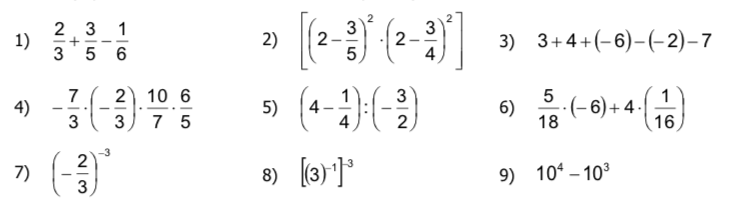
\includegraphics[scale=0.6]{test-form-1}
%
%}
\begin{minipage}{\linewidth}
	\begin{multicols}{2}
		\begin{parts}
			\part
			\exonly{$\frac{3}{3}+\frac{3}{5}-\frac{1}{6}$ }
			\solonly{$\frac{11}{10}$ }
			
			\part
			\exonly{ $\left[ \left( 2-\frac{3}{5}\right) ^2 \cdot \left( 2-\frac{3}{4}\right) ^2 \right] $  }
			\solonly{$\frac{49}{16}$ }
			
			\part
			\exonly{$3+4+(-6)-(-2)-7$ }
			\solonly{$-4$ }
			
			\part
			\exonly{$-\frac{7}{3} \cdot \left( -\frac{2}{3}\right) \cdot \frac{10}{7} \cdot \frac{6}{5} $ }
			\solonly{$\frac{8}{3}$ }
			
			\part
			\exonly{$\left( 4-\frac{1}{4}\right) \div \left( -\frac{3}{2}\right) $ }
			\solonly{$-\frac{5}{2}$ }
			
			\part
			\exonly{$\frac{15}{18}\cdot\left( -6 \right) +4\cdot \left( \frac{1}{16}\right) $ }
			\solonly{$-\frac{17}{12}$ }
			
			\part
			\exonly{$\left( -\frac{2}{3}\right) ^{-3}$ }
			\solonly{$-\frac{27}{8}$ }
			
			\part
			\exonly{$\left[ \left( 3\right) ^{-1}\right] ^{-3}$ }
			\solonly{$27$ }
			
			\part
			\exonly{$10^4-10^3$ }
			\solonly{$9000$ }
		\end{parts}
	\end{multicols}
\end{minipage}

%\solonly{
%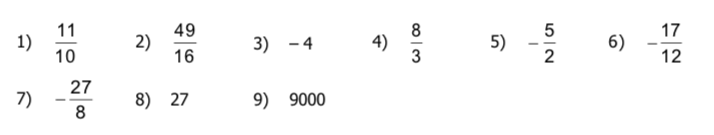
\includegraphics[scale=0.6]{test-form-1-sol}
%}

%\exnewpage

\begin{minipage}{\textwidth}	
	\question
	\exonly{Calcola senza aiutarti con la calcolatrice:}
		
	\begin{minipage}{\linewidth}
		\begin{multicols}{2}
			\begin{parts}
				
				\part 
				\exonly{$ x - 2x + 3x - 4x + 5x - 6x =$ }
				\solonly{$ -3x$ }
				
				\part 
				\exonly{$ a^2 + 2a -3a^2 +a = $ }
				\solonly{$-2a^2+3a$ }
				
				\part
				\exonly{$ a^2 \cdot a^3 = $ }
				\solonly{$a^5$ }
				\part 
				\exonly{$ \left(a^2\right)^2 + a\cdot a^3 - \left(a^6\right)^{-2} =$ }
				\solonly{$\dfrac{2a^{16}-1}{a^{12}}$ }
				
				\part 
				\exonly{$ x^{-2} \cdot \left(x^2\right)^3 = $ }
				\solonly{$x^4$ }
				
				\part 
				\exonly{$ \dfrac{9 \cdot a^2 \cdot b^3 }{3 \cdot a^{-2} \cdot b^5} = $ }
				\solonly{$\dfrac{3a^4}{b^2}$ }
				
				\part 
				\exonly{$ \dfrac{2 \cdot a^3 \cdot b^2 }{3 \cdot a \cdot b^4} \cdot \dfrac{a+b}{a}  = $ }
				\solonly{$\dfrac{2a^2+2ab}{3b^2}$ }
				
				\part 
				\exonly{$ a\left(a(a^{-1}+1) + a(a-1)\right) =$ }
				\solonly{$ a^3+a$ }
			\end{parts}
			
		\end{multicols}
		
\end{minipage}
\end{minipage}


\end{questions}

\subsection{Notazione scientifica}
\begin{questions}

\question
\exonly{Esprimi la tua altezza in notazione scientifica}
\solonly{Esempio con \SI{178}{\centi\metre} }

	\begin{multicols}{2}
		\begin{parts}
			\part 
			\exonly{in metri }
			\solonly{ \SI{1.78}{\metre} }
			\part 
			\exonly{in centimetri }
			\solonly{\SI{1.78e2}{\centi\metre} }
			\part 
			\exonly{in millimetri }
			\solonly{\SI{1.78e3}{\milli\metre} }
			\part 
			\exonly{in chilometri }
			\solonly{\SI{1.78e-3}{\kilo\metre} } 
			\part 
			\exonly{in pollici ($\SI{1}{in}=\SI{2.54}{cm}$) }
			\solonly{\SI{7.01e1}{in} }
			\part 
			\exonly{in piedi ($\SI{1}{ft}=\SI{12}{in}$) }
			\solonly{\SI{5.84}{ft} }
		\end{parts}
	\end{multicols}


\question
\exonly{Calcola senza aiutarti con la calcolatrice:}

	\begin{parts}
		\part 
		\exonly{$\num{2e3} + \num{5e2} +\num{3e1}=$ }
		\solonly{\num{2530}=\num{2.53e3} }
		\part
		\exonly{ $\num{3e3} + \num{5e-2} +\num{2e-1} + \num{6e1} + \num{4e0} + \num{9e2} + 7 \times 10^0=$ }
		\solonly{\num{3971.25} }
		
		\part 
		\exonly{$ \num{12e3} \times \num{2e-3} \times \num{3e-6} =$ }
		\solonly{\num{72e-6}=\num{7.2e-5} }
		
		\part 
		\exonly{$ \dfrac{\num{12e3}+ 500}{\num{5e6}} = $ }
		\solonly{ \num{2.5e-3}  }
		
		\part 
		\exonly{$ \dfrac{\num{2e-2} \times\num{3e1} \times\num{4e2}}{\num{4e2} \times\num{6e-3} \times\num{2e1}} =$ }
		\solonly{ \num{5}}
		
	\end{parts}

\question
\exonly{ Calcolare le seguenti espressioni ed esprimere il risultato in notazione scientifica }

\begin{minipage}{\linewidth}
	\begin{multicols}{2}
		\begin{parts}
			\part
			\exonly{ $\num{0.5e-1 }$ }
			\solonly{$ \num{5e-2}$ }
			
			\part
			\exonly{ $\num{-6.5e-5} -\num{3.5e-7} $ }
			\solonly{$-\num{6.535e-5} $ }
			
			\part
			\exonly{$\left(3 \cdot 10^{-2}\right)\left(4 \cdot 10^{-1}\right)$ }
			\solonly{ $\num{1.2e-2}$ }
			
			\part
			\exonly{$8^{2} \cdot 10^{-2}$ }
			\solonly{$\num{6.4e-1} $ }
			
			\part
			\exonly{ $200 \cdot 10^{4}$ }
			\solonly{$\num{2e6}$ }
			
			\part
			\exonly{$\left(5 \cdot 10^{-4}\right)\left(0,7 \cdot 10^{-8}\right)$ }
			\solonly{$\num{3.5e-12} $ }
			
			\part
			\exonly{$\left(7 \cdot 10^{-7}\right)^{2}$ }
			\solonly{$\num{4.9e-13}$ }
			
			\part
			\exonly{ $\left(3^{2} \cdot 10^{-6}\right)^{2} \cdot 10$ }
			\solonly{$ \num{8.1e-10} $ }
			
			\part
			\exonly{$10^{4}-10^{3}$ }
			\solonly{$\num{9e3}$ }
			
			\part
			\exonly{ $\left(0,4 \cdot 10^{-4}\right)(0,8) \cdot 10^{-4}$}
			\solonly{$\num{3.2e-9}$ }
			
			\part
			\exonly{$10^{5}-10^{-5}$ }
			\solonly{$\num{9.999999999e4}$ }
			
			\part
			\exonly{$\frac{\left(4^{2}\right)^{-2} \cdot 10^{-3}}{4^{-2} \cdot 10^{-8}}$ }
			\solonly{ $\num{6.25e3}$ }
			
			\part
			\exonly{$-\num{4.2e-3}+\num{4.2e5}$ }
			\solonly{$\num{4.199999958e5} $ }
		\end{parts}
	\end{multicols}
\end{minipage}

\question
\exonly{Calcola ed esprimi il risalutato tenendo conto delle cifre significative delle misure:}

\begin{minipage}{\linewidth}
	\begin{multicols}{2}
		\begin{parts}
			\part 
			\exonly{$ \SI{5.3}{cm} - \SI{3.2}{mm} = $  }
			\solonly{\SI{50}{\milli\metre}=\SI{5.0}{\centi\metre} }
			\part 
			\exonly{$ \SI{43.5}{cm} \cdot \SI{9.3}{mm} = $  }
			\solonly{\SI{4.0e1}{\square\centi\metre}=\SI{4.0e3}{\square\milli\metre} }
			\part
			\exonly{ $ \SI{9.2}{cm^2} + \SI{123}{mm^2} = $  }
			\solonly{ \SI{1.0e3}{\square\milli\metre} }
			\part
			\exonly{ $ \dfrac{\SI{430}{mm^2}}{\SI{3.2}{cm}} = $ }
			\solonly{$\SI{1.3e1}{mm^2}$ }
			\part 
			\exonly{$ \SI{3.2}{k\ohm} \cdot \SI{15}{mA} = $ }
			\solonly{$\SI{48}{V}$ }
			\part 
			\exonly{$ \dfrac{\SI{12}{V}}{\SI{60}{mA}} = $ }
			\solonly{\SI{2.0e2}{\ohm} }
		\end{parts}
	\end{multicols}
\end{minipage}

\question
\exonly{
	Esprimi le seguenti frazioni in notazione scientifica e tecnica tendendo conto delle cifre significative }

\begin{minipage}{\linewidth}
	\begin{multicols}{2}
		\begin{parts}
			\setlength\itemsep{1em}
			\part 
			\exonly{$\frac{5}{8}$ }
			\solonly{\num{6e-1} \\ \num{600e-3} }
			\part 
			\exonly{$\frac{724}{5}$ }
			\solonly{\solonly{\num{1e2} \\ \num{100e0} } }
			\part 
			\exonly{$\frac{11562}{470000}$ }
			\solonly{\num{2.5e-2} \\ \num{25e-3} } 
			
			\part 
			\exonly{$\frac{123456}{7}$ }
			\solonly{ \num{2e4} \\ \num{20e3}  }
			
			\part
			\exonly{ $\frac{12}{16500}$= }
			\solonly{\num{7.3e-3} \\ \num{7.3e-3}  }
			
			\part 
			\exonly{$\frac{146}{2420}$= }
			\solonly{\num{6.03e-2} \\ \num{60.3e-3}  }
		\end{parts}
	\end{multicols}
\end{minipage}


\end{questions}
\section{Modelli di primo  grado}

\subsection{Invertire formule}
\begin{questions}

	\begin{qblock}

		\question
		\exonly{Legge oraria del moto rettilineo uniforme MRU

			\begin{equation*}
				x=v \cdot t + x_0
			\end{equation*}

			\begin{center}
				\renewcommand\arraystretch{1.2}
				\begin{tabular}{lll}
					\hline
					variabile & grandezza          & unità di misura    \\
					\hline
					$x$       & posizione          & $\si{m}$           \\
					$v$       & velocità           & $\si{\frac{m}{s}}$ \\
					$t$       & tempo trascorso    & $\si{s}$           \\
					$x_o$     & posizione iniziale & $\si{m}$           \\
					\hline
				\end{tabular}
			\end{center}
		}


		\begin{parts}
			\part \exonly{Trova la formula per calcolare ogni variabile in funzione delle altre }

			$v  =  \solonly{\dfrac{x-x_0}{t} }$ \\
			$	t  = \solonly{\dfrac{x-x_0}{v} }$ \\
			$	x_0  = \solonly{x-vt}
			$




			\part \exonly{Calcola i valori mancanti nella seguente tabella }

			\bigskip

			\renewcommand\arraystretch{2.2}
			\begin{tabular}{|C{3cm}|C{3cm}|C{3cm}|C{3cm}|}
				\hline
				$x$                           & $v$                                     & $t$                       & $x_o$                      \\
				\hline
				\solonly{\SI{41.5}{\metre}  } & $\SI{3}{\frac{m}{s}}$                   & $\SI{13}{s}$              & $\SI{2.5}{m}$              \\
				%		\midrule
				$\SI{23}{km}$                 & \solonly{$\SI{5.94}{\frac{km}{h}}  $  } & $\SI{3.2}{h}$             & $\SI{4}{km}$               \\
				%		\midrule
				$\SI{173}{m}$                 & $\SI{2.7}{\frac{m}{s}}$                 & \solonly{$\SI{48.5}{s}$ } & $\SI{42}{m}$               \\
				%		\midrule
				$\SI{236}{km}$                & $\SI{123}{\frac{km}{h}}$                & $\SI{5}{h}$               & \solonly{$\SI{-379}{km}$ } \\
				%		\midrule
				$\SI{1323}{m}$                & \solonly{$\SI{21.77}{\frac{m}{min}}$ }  & $\SI{47}{min}$            & $\SI{300}{m}$              \\
				\hline
			\end{tabular}

		\end{parts}
	\end{qblock}

	\begin{qblock}
		\question
		\exonly{Resistenza di un conduttore
			\nopagebreak
			\begin{equation*}
				R=\dfrac{\rho \cdot l}{A}
			\end{equation*}
			\nopagebreak

			\begin{center}
				\renewcommand\arraystretch{1.2}
				\begin{tabular}{lll}
					\hline
					variabile & grandezza                 & unità di misura                  \\
					\hline
					$R$       & resistenza del conduttore & $\si{\ohm}$                      \\
					$\rho$    & resistività del materiale & $\si{\frac{\ohm \cdot mm^2}{m}}$ \\
					$l$       & lunghezza del conduttore  & $\si{m}$                         \\
					$A$       & sezione del conduttore    & $\si{mm^2}$                      \\
					\hline
				\end{tabular}
			\end{center}
		}


		\begin{parts}
			\part  \exonly{Trova la formula per calcolare ogni variabile in funzione delle altre }

			$\rho= \solonly{\dfrac{AR}{l} }$\\
			$l=\solonly{\dfrac{AR}{\rho} }$\\
			$A=\solonly{\dfrac{\rho l }R }$

			\nopagebreak

			\part \exonly{Calcola i valori mancanti nella seguente tabella }

			\bigskip

			\renewcommand\arraystretch{2.2}
			\begin{tabular}{|C{3cm}|C{3cm}|C{3cm}|C{3cm}|}
				\hline
				$R$                          & $\rho$                                               & $l$                            & $A$                            \\
				\hline
				\solonly{$\SI{8.75}{\ohm} $} & $\SI{0.0175}{\frac{\ohm \cdot mm^2}{m}}$             & $\SI{250}{m}$                  & $\SI{0.5}{mm^2}$               \\
				%		\midrule
				$\SI{10}{\ohm}$              & \solonly{$\SI{0.017}{\frac{\ohm \cdot mm^2}{m}}$  }  & $\SI{1.5}{km}$                 & $\SI{2.5}{mm^2}$               \\
				%		\midrule
				$\SI{152}{m\ohm}$            & $\SI{0.0287}{\frac{\ohm \cdot mm^2}{m}}$             & \solonly{$\SI{2.12}{\metre}$ } & $\SI{0.4}{mm^2}$               \\
				%		\midrule
				$\SI{0.5}{\ohm}$             & $\SI{0.0175}{\frac{\ohm \cdot mm^2}{m}}$             & $\SI{3.5}{km}$                 & \solonly{ $\SI{122.5}{mm^2}$ } \\
				%		\midrule
				$\SI{2}{\ohm}$               & \solonly{$\SI{0.0286}{\frac{\ohm \cdot mm^2}{m}}$  } & $\SI{105}{m}$                  & $\SI{1.5}{mm^2}$               \\
				\hline
			\end{tabular}

		\end{parts}
	\end{qblock}

\end{questions}

\subsection{Equazioni e sistemi di primo grado}
\begin{questions}

	\begin{qblock}
		\question

		\exonly{ Risolvi le seguenti equazioni: }
		\begin{parts}
			\setlength\itemsep{3mm}
			\item
			\exonly{$x-3=2$ }
			\solonly{$\es{5}$}

			\item \exonly{$3x=9$ } \solonly{$\es{3 }$}
			\item \exonly{$2x+3=7$ } \solonly{$\es{2 }$ }
			\item \exonly{$3x-5=7-x$ } \solonly{$\es{3 }$ }
			\item \exonly{$3x+2=5$ } \solonly{$\es{1 }$ }
			\item \exonly{$5x+3=2x-7$ } \solonly{$\es{-\frac{10}{3} }$ }
			\item \exonly{$2x+3-7x=3x-5+2x-1$ } \solonly{$\es{\frac{9}{10} }$ }
		\end{parts}
	\end{qblock}

	\begin{qblock}
		\question
		\exonly{Risolvi le seguenti equazioni: }

		\begin{parts}
			\setlength\itemsep{3mm}
			\item \exonly{$2(3x-2)+3(x-1)=4(x-1)-(3-x)$ }
			\solonly{$\es{0 }$ }

			\item \exonly{$\frac{2}{3}(5x+3)-2(\frac{1}{3}x-\frac{3}{4})=\frac{1}{2}(\frac{3}{5}-\frac{3}{7}x)$ }
			\solonly{$\es{-\frac{672}{605} }$ }

			\item \exonly{$3(x-5)+2(3-2x)=x+3-2(x-4)$ }
			\solonly{$S=\emptyset$ }

			\item \exonly{$(x+3)(x-2)=x(x+3)-3(x-4)$ }
			\solonly{$\es{18 }$ }
			\item \exonly{$2(3x-4)=4(x+1)+2(x-6)$ }
			\solonly{$S=\R$ }
		\end{parts}
	\end{qblock}

	\begin{qblock}
		\question
		\exonly{ Risolvi le seguenti equazioni nell'incognita $x$ e discuti le soluzioni in funzione del parametro $a$: }

		\begin{parts}
			\setlength\itemsep{3mm}
			\item \exonly{$2x+3-2a=3x-5+2a-1$ } \solonly{$\es{9-4a \mid a \in \R }$ }
			\item \exonly{$2(3x-2a)+3(x-a)=4(x-a)-(3a-x)$ } \solonly{$\es{0 \mid a \in \R }$ }
			\item \exonly{$3(x-5a)+2(3-2x)=x+3-2(x-4a)$ } \solonly{Se $a=\frac{3}{23}$: $S=\R$, se $a\neq\frac{3}{23}$: $S=\emptyset$ }
			\item \exonly{$(x+3)(x-a)=x(x+2a)-3(x-4)$ } \solonly{$\es{\frac{a+4}{2-a} \mid a \neq 2 }$ , se $a=2$: $S=\emptyset$ }
		\end{parts}

	\end{qblock}

	\begin{qblock}
		\question
		\exonly{Risolvere i seguenti sistemi. }


		\begin{multicols}{2}
			\begin{parts}
				\setlength\itemsep{3mm}

				\item
				\exonly{$
						\left\{
						\begin{aligned}
							x+3 & = 3x-1 \\
							x-y & = 5
						\end{aligned}
						\right. $ }
				\solonly{$\es{\left(2;-2\right)}$ }

				\item
				\exonly{ $
						\left\{
						\begin{aligned}
							2x-3  & = 4-5x \\
							3x-2y & = 2
						\end{aligned}
						\right. $ }
				\solonly{$\es{\left( 1;\frac{1}{2}\right)  }$ }

				\item
				\exonly{$
						\left\{
						\begin{aligned}
							2x-4  & = 3 \\
							-x+2y & = 5
						\end{aligned}
						\right. $ }
				\solonly{$\es{\left( \frac{7}{2};\frac{17}{4}\right) }$ }




				\item
				\exonly{$
						\left\{
						\begin{aligned}
							5x-5   & = 1  \\
							-6x+9y & = -3
						\end{aligned}
						\right. $ }

				\solonly{$\es{\left( \frac{6}{5};\frac{7}{15}\right)  }$ }
			\end{parts}
		\end{multicols}
	\end{qblock}

	\begin{qblock}
		\question
		\exonly{Risolvere i  seguenti sistemi e indicare l'insieme delle soluzioni. }
		\begin{multicols}{2}
			\begin{parts}
				\setlength\itemsep{3mm}
				\item
				\exonly{
					$\left\{
						\begin{aligned}
							3x-y  & = 2 \\
							2x-5y & = 4
						\end{aligned}
						\right. $
				}

				\solonly{
					$\es{\left( \frac{6}{13};-\frac{8}{13}\right)  }$
				}

				\item
				\exonly{$
						\left\{
						\begin{aligned}
							x+3y  & = 3  \\
							2x+4y & = -8
						\end{aligned}
						\right. $ }

				\solonly{
					$\es{\left( -18;7\right)  }$
				}
				\item \exonly{$
						\left\{
						\begin{aligned}
							2x-3y & = 1 \\
							2x-5y & = 4
						\end{aligned}
						\right. $ }

				\solonly{
					$\es{\left( -\frac{7}{4};-\frac{3}{2}\right)  }$
				}
				\item
				\exonly{$
						\left\{
						\begin{aligned}
							3x+3y & = 3  \\
							2x-3y & = -2
						\end{aligned}
						\right. $ }

				\solonly{
					$\es{\left( \frac{1}{5};\frac{4}{5}\right)  }$
				}

				\item \exonly{$
						\left\{
						\begin{aligned}
							4x-3  & = 2 \\
							2x-6y & = 4
						\end{aligned}
						\right. $ }

				\solonly{
					$\es{\left( \frac{5}{4};-\frac{1}{4}\right)  }$
				}

				\item \exonly{$
						\left\{
						\begin{aligned}
							2x+3y & = 3  \\
							6x+4y & = -3
						\end{aligned}
						\right. $ }

				\solonly{
					$\es{\left(- \frac{21}{10};\frac{12}{5}\right)  }$
				}

				\item \exonly{$
						\left\{
						\begin{aligned}
							3x-4y & = 6  \\
							2x-3y & = -8
						\end{aligned}
						\right. $ }

				\solonly{
					$\es{\left(-14;-12\right)  }$
				}
				\item \exonly{$
						\left\{
						\begin{aligned}
							4x+5y & = 3  \\
							2x+7y & = -8
						\end{aligned}
						\right. $ }

				\solonly{
					$\es{\left(\frac{61}{18};-\frac{19}{9}\right)  }$
				}



			\end{parts}
		\end{multicols}
	\end{qblock}

	\begin{qblock}

		\question
		\exonly{Risolvere i seguenti sistemi e indicare l'insieme delle soluzioni discutendo le soluzioni in funzione del parametro $a$.}

		\begin{parts}
			\item \exonly{$
					\left\{
					\begin{aligned}
						3x+5y & = -2a \\
						x+4y  & = 4
					\end{aligned}
					\right. $	 }

			\solonly{
				$\es{\left(- \frac{8a+20}{7};\frac{2a+12}{7}\right) \mid a \in \R }$
			}

			\item\exonly{ $
					\left\{
					\begin{aligned}
						2x+a\cdot y & = -6 \\
						2x-7y       & = -a
					\end{aligned}
					\right. $ }

			\solonly{
				Se $a \neq -7$: 	$\es{\left(\frac{-a^2 - 42}{2a+14}; \frac{a-6}{a+7}\right) }$  \\
				Se $a = -7$: 	$S=\emptyset $  \\
			}



		\end{parts}
	\end{qblock}

	\begin{qblock}
		\question
		\exonly{Risolvere i seguenti sistemi}

		\begin{multicols}{2}
			\begin{parts}
				\part
				\exonly{$
						\left\{
						\begin{aligned}
							x+y+z  & = 3  \\
							x-y-z  & = 4  \\
							-x+y-z & = -2
						\end{aligned}
						\right. $ }

				\solonly{$\es{\left(\frac{7}{2}; \frac{1}{2};-1\right) }$   }


				\part
				\exonly{ $
						\left\{
						\begin{aligned}
							3x-4y+z  & = 2  \\
							2x+2y-3z & = 1  \\
							3x-3y+2z & = -2
						\end{aligned}
						\right. $ }

				\solonly{$\es{\left(-1; -\frac{9}{5};-\frac{11}{5}\right) }$   }

				\part
				\exonly{ $
						\left\{
						\begin{aligned}
							2x - 3y + z & =  x -  y - z \\
							x + 2y - z  & =  2 - 3x     \\
							2x + 4y +3z & = -x +z + 1
						\end{aligned}
						\right. $ }

				\solonly{$\es{\left(\frac{11}{25}; \frac{1}{50};-\frac{1}{5}\right) }$   }

			\end{parts}
		\end{multicols}
	\end{qblock}
\end{questions}


\subsection{Funzioni e rappresentazione grafica }
\begin{questions}

	\begin{qblock}

		\question
		\exonly{Determinare la legge di assegnazione (l'equazione) delle rette) $a$, $b$, $c$, $d$ et $e$. }

		%\includegraphics[scale=1]{ex-eq-droites-rev.png}
		\exonly{
			\begin{tikzpicture}
				\begin{axis}[
						AxisDefaults,
						SmallAxisLabels,
						width=0.75\linewidth,
						domain=-6:10,
						restrict y to domain=-5:8,
						xmin=-6,xmax=10, ymin=-4, ymax=7,
					]
					\addplot[]{5*x/2+3/2} node[above left, pos=0.8] {$a$} ;
					\addplot[]{-5*x/6+7/3}node[above, pos=0.15] {$b$} ;
					\addplot[]{2}node[above, pos=0.2] {$c$} ;
					\addplot[]{7*x/3-37/3}node[ right, pos=0.8] {$d$} ;
					\addplot[]{-9*x/5+66/5}node[above right, pos=0.2] {$e$} ;
				\end{axis}
			\end{tikzpicture} }

		\solonly{


			\begin{multicols}{2}
				\begin{enumerate}[a)]
					\item $y=\frac{5}{2}x+\frac{3}{2}$
					\item $y=-\frac{5}{6}x+\frac{7}{3}$
					\item $y=2$
					\item $y=\frac{7}{3}x-\frac{37}{3}$
					\item $y=-\frac{9}{5}x+\frac{66}{5}$

				\end{enumerate}
			\end{multicols}

		}
	\end{qblock}

	\begin{qblock}
		\question
		\exonly{Determinare la legge di assegnazione (equazioni) delle rette qui sotto: }


		\exonly{\begin{tikzpicture}
				\begin{axis}[
						AxisDefaults,
						SmallAxisLabels,
						width=0.75\linewidth,
						domain=-8:10,
						restrict y to domain=-8:8,
						ymin=-6, ymax=7, %set the min and max y tick
						xmin=-8, xmax=10,  %set the min and max x tick
					]
					\addplot[black]{-5*\x/6+1} node[above,pos=0.1] {$a$};
					\addplot[black]{\x/5-4} node[above,pos=0.8] {$b$};
					\addplot[black]{\x+4} node[right,pos=0.9] {$c$};
					\addplot[black]{2*\x/5-3} node[above,pos=0.9] {$d$};
					\addplot[black]{-6*\x +6} node[right,pos=0.8] {$e$};
				\end{axis}
			\end{tikzpicture} }


		\solonly{
			\begin{multicols}{2}


				\begin{enumerate}[a)]
					\item   $y= -\frac{5}{6}x+1$

					\item  $y=\frac{1}{5}x-4$

					\item  $y= x+4$
					\item  $y=\frac{2}{5}x-3$
					\item  $y=-6x+6 $
				\end{enumerate}
			\end{multicols}
		}
	\end{qblock}

	\begin{qblock}
		\question
		\exonly{Determinare l'equazione della retta passante per  A(-3;5) e B(-2;1). }

		\solonly{$y=-4x-7$}
	\end{qblock}

	\begin{qblock}
		\question
		\exonly{Determinare l'equazione della retta passante per A(-3;-8) e B(3;1). }

		\solonly{$y=\dfrac{3}{2}x-\dfrac{7}{2}$}
	\end{qblock}

	\begin{qblock}
		\question
		\exonly{Determinare l'equazione della retta passante per A($\frac{3}{4}$;1) e B(1;3). }

		\solonly{$y=8x-5$}
	\end{qblock}

	\begin{qblock}
		\question
		\exonly{Determinare l'equazione della retta passante per  A(4;1)  avente pendenza $m= \dfrac{1}{3}$. }

		\solonly{$y=\dfrac{1}{3}x-\dfrac{1}{3}$}
	\end{qblock}

	\begin{qblock}
		\question
		\exonly{Qual'é la pendenza della retta di equazione  $12x = 4y -1$? Qual'é la sua ordinata all'origine? }

		\solonly{
			Pendenza: $m=3$\\
			Ordinata all'origine: $b=\frac{1}{4}$
		}
	\end{qblock}

	\begin{qblock}
		\question
		\exonly{Determinare l'equazione della retta passante per  A(-2;1) che sia parallela alla retta di equazione  $21y+42x=7$. }

		\solonly{$y= -2x-3$}

		\question
		\exonly{Determinare l'equazione della retta passante per  A(-5;5) che sia perpendicolare alla retta di equazione  $3y-7x+4=0$. }

		\solonly{$y= -\frac{3}{7}x+\frac{20}{7}$}

	\end{qblock}

	\begin{qblock}
		\question

		\exonly{Determinare i punti d'intersezione della retta di equazione $5x + 6y = 8$ con : }

		\begin{parts}
			\part
			\exonly{l'asse delle ascisse $x$ }
			\solonly{Asse  x: $y=0 \Rightarrow \left( \frac{8}{5};0\right) $ }
			\part
			\exonly{l'asse delle ordinate $y$ }
			\solonly{Asse y: $x=0 \Rightarrow \left( 0;\frac{4}{3}\right) $ }
		\end{parts}
	\end{qblock}

	\begin{qblock}


		\question
		\exonly{Determinare i punti d'intersezione della retta di equazione $6x - 3y = 16$ con: }

		\begin{parts}
			\part \exonly{l'asse delle ascisse $x$ } \solonly{$\left( \dfrac{8}{3};0\right)$ }
			\part  \exonly{l'asse delle ordinate $y$ } \solonly{$\left( 0;-\dfrac{16}{3}\right) $ }
			\part \exonly{la retta di equazione  $y=4x-3$ } \solonly{$\left( -\dfrac{7}{6};-\dfrac{23}{3}\right) $ }
			\part \exonly{la retta di equazione $5x + 6y = 8$ } \solonly{$\left( \dfrac{40}{17};-\dfrac{32}{51}\right) $ }
		\end{parts}
	\end{qblock}

\end{questions}

\subsection{Problemi}
\begin{questions}

	\begin{qblock}
		\question
		\exonly{Gérard si é appena trasferito  dal canton Friburgo e vuole provare ad importare la famosa "double crème de la Gruyère" in Ticino. Ha calcolato che i suo costi fissi quotidiani sono di \SI{64 }{\CHF} e che ogni confezione di "double crème" gli costa \SI{12}{\CHF}. Gérard decide di vendere ad un prezzo di \SI{20}{\CHF} la confezione da mezzo chilo. }

		\begin{parts}
			\part
			\exonly{ Quante confezioni dovrebbe vedere in media al giorno per coprire i  costi. }

			\solonly{ Dovrebbe vendere almeno 8 confezioni.}

			\nopagebreak
			\exonly{\uplevel{
					Un rappresentante di propone a Gérard un nuova macchina per gestire l'imballaggio. Se decidesse di investire in questa innovazione i suoi costi fissi salirebbero a \SI{144}{\CHF} ma in compenso il costo per confezione scenderebbe a \SI{8}{\CHF}. Gérard vuole sempre vendere a \SI{20}{\CHF} ogni confezione.
				} }
			\part
			\exonly{Quali scenari si presentano a Gérard e quale decisione dovrebbe prendere in funzione del numero di confezione vendute, in media, quotidianamente. }

			\solonly{$<8:$ chiudere \\ $8\leq x \leq 20$: mantenere sistema attuale \\ $x>20$: rinnovare il sistema di imballaggio }

		\end{parts}
	\end{qblock}

	\begin{qblock}
		\question
		\exonly{
			Seicento persone hanno assistito ad uno spettacolo teatrale. I prezzi dei biglietti erano di \SI{5}{\CHF} per gli adulti e di \SI{2}{\CHF} per i bambini.
			A fine rappresentazione in cassa ci  sono \SI{2400}{\CHF}.
			Quanti adulti e quanti bambini hanno assistito alla rappresentazione?
			%Six cents personnes assistent à la première d'un film. Les billets pour adultes coûtent \SI{5}{\CHF}, et les enfants sont admis pour \SI{2}{\CHF}. Si la caisse contient \SI{2400}{\CHF}, combien d'enfants assistaient à la première? 

		}
		\solonly{
			$200$ bambini e $400$ adulti.
		}
	\end{qblock}

	\begin{qblock}
		\question
		\exonly{
			Nell'ambito di un test medico che mira a misurare la tolleranza ai carboidrati si somministrano ad un adulto \SI{7}{\centi\litre}  di una soluzione con una concentrazione del 30\% di glucosio.

			\nopagebreak
			Una tale concentrazione non é applicabile nel caso debba essere somministrata ad un bambino. Per un bambino bisognerebbe somministrare \SI{7}{\centi\litre} ad una concentrazione del 20\%.

			\nopagebreak
			Quanta soluzione per adulti bisognerà diluire per ottenere tale scopo?
		}
		\solonly{
			$\dfrac{14}{3}\approx \SI{4.67}{\centi\litre}$ de soluzione e $\dfrac{7}{3} \approx \SI{2.33}{\centi\litre}$ d'acqua.
		}
	\end{qblock}

	\begin{qblock}
		\question
		\exonly{

			Un farmacista deve preparare \SI{15}{\milli\litre} di gocce speciali per gli occhi per un paziente affetto da glaucoma.
			La soluzione deve contenere il 2\% di un particolare principio attivo ma il farmacista ne ha attualmente in stock solo in soluzione. Una soluzione al 10\% e una all'1\%.
			\nopagebreak

			Quali quantità delle due soluzioni deve utilizzare per soddisfare la prescrizione del medico?

		}
		\solonly{
			$\dfrac{5}{3}\approx \SI{1.67}{\milli\litre}$ della soluzione al 10\% e $\dfrac{40}{3}\approx \SI{13.33}{\milli\litre}$  all'1\%
		}

	\end{qblock}

	\begin{qblock}


		\question \exonly{
			Abbiamo a disposizione una grande quantità di una lega rame--argento al \num{7.5}\% di rame e del rame puro.

			\nopagebreak
			Quanti grammi di questa lega e quanti grammi di rame deve mischiare per preparare \SI{200}{\gram} di una lega rame--argento al 10\% di rame?
			%Combien de grammes de cuivre pur et combien de grammes d'alliage de la %livre devrait-on utiliser pour préparer \SI{200}{\gram}  d'alliage cuivre--argent à 10\% de cuivre ?

		}
		\solonly{
			\SI{194.6}{\gram} di lega e \SI{5.4}{\gram} di rame puro.
		}
	\end{qblock}

	\begin{qblock}

		\question \exonly{
			Un corridore comincia  un percorso di allenamento e corre alla velocità costante di \SI{9.7}{\kilo\meter/\hour}.
			Cinque minuti più tardi un secondo corridore comincia lo stesso percorso ma corre alla velocità costante di  \SI{12.9}{\kilo\meter/\hour}.

			\nopagebreak
			Quanto tempo occorre al secondo corridore per raggiungere il primo?

			%Dopo quanto tempo il secondo corridore raggiungerà il primo?
			%
			%Un coureur part du début d'un parcours d'entraînement et court à la vitesse constante de \SI{9.7}{\kilo\meter/\hour}. 
			%Cinq minutes plus tard, un autre coureur part du même point, il court à \SI{12.9}{\kilo\meter/\hour} et suit le même chemin. 
			%
			%Combien de temps faudra-t-il au second coureur pour rattraper le premier ? 

		}
		\solonly{
			Il secondo corridore raggiungerà il primo dopo aver corso ca. 15 minuti.
			%Le second coureur nécessitera ca. 20 minutes pour rattraper le premier.
		}
	\end{qblock}

	\begin{qblock}
		\question
		\exonly{
			Eduardo deve camminare \SI{3}{\kilo\meter} per raggiungere la casa del suo amici Jason.
			Al ritorno, Eduardo, prende in prestito la bicicletta di Jason. La sua velocità media in bicicletta supera di  \SI{4}{\kilo\meter/\hour}  quella a piedi e Eduardo impiega in tutto \SI{2}{\hour}  per il tragitto andata e ritorno.

			A quale velocità cammina Eduardo?

			%Quali sono le velocità nei due tragitti (a piedi e in bicicletta)?
			%
			%
			%Depuis ça maison Édouard doit marcher pendant \SI{3}{\kilo\meter} pour aller chez son copain Jason. \\
			%Pour le trajet de retour il emprunte le vélo de Jason. Sa vitesse moyenne à vélo est de \SI{4}{\kilo\meter/\hour} plus rapide qu'en marchant et il a mesuré que l'allez--retour lui à pris \SI{2}{\hour} en tout. \\
			%Quelle est la vitesse moyenne de marche de   Édouard?
		}

		\solonly{
			Eduardo cammina ad una velocità di \SI{2}{\kilo\meter/\hour}

		}
	\end{qblock}


	\begin{qblock}
		\question
		\exonly{La città A dista 40 km dalla città B e questa dista 160 km dalla città C  Un'automobile parte da B diretta verso C, viaggiando a velocità costante. Contemporaneamente parte da A una seconda automobile che viaggia ad una velocità costante superiore di 20 km/h a quella della prima auto e, passando per B, giunge in C contemporaneamente alla prima auto.

			Determina le velocità delle due auto.}

		\solonly{80 e 100 Km/h}
	\end{qblock}


	\begin{qblock}
		\question \exonly{
			Abbiamo a disposizione due tubi da utilizzare per il riempimento di una piscina. Uno di piccola portata con il quale sappiamo di poter riempire la piscina in 8 ore. Il secondo tubo di maggiore portata ci permetterebbe di riempire la piscina in 5 ore.

			In quanto tempo potremmo riempire la piscina utilizzandoli contemporaneamente?
			%Utilizzando u
			%Avec un tuyau d'arrosage, une piscine peut être remplie en 8 heures. Avec un autre tuyau plus gros, employé seul, on la remplit en 5 heures. 
			%
			%En combien de temps remplira-t-on la piscine en employant simultanément les deux tuyaux ?

		}
		\solonly{
			$\frac{40}{13}\approx \SI{3.08}{\hour}$.

		}
	\end{qblock}


	\begin{qblock}
		\question \exonly{
			Un conducente effettua lo stesso tragitto di \SI{120}{\kilo\meter} una volta di giorno e una volta di notte.
			Constata così che di notte impiega 36 minuti in meno che di giorno e che la sua velocità media é di \SI{10}{\kilo\meter / \hour} superiore a quelle di giorno.

			Qual'é la sua velocità media di giorno?

		}

		\solonly{

			\SI{40}{\kilo\meter / \hour}.


		}
	\end{qblock}

\end{questions}

\end{document}